% This is LLNCS.DEM the demonstration file of
% the LaTeX macro package from Springer-Verlag
% for Lecture Notes in Computer Science,
% version 2.4 for LaTeX2e as of 16. April 2010
%
\documentclass{llncs}
%
\usepackage{makeidx}  % allows for indexgeneration
\usepackage[pdftex]{graphicx}
%
\begin{document}
%
\mainmatter              % start of the contributions
%
\title{The importance of Opposites}
%
\titlerunning{The importance of Opposites}  % abbreviated title (for running head)
%                                     also used for the TOC unless
%                                     \toctitle is used
%
\author{Edward D. Willink\inst{1}}
%
\authorrunning{Edward Willink} % abbreviated author list (for running head)
%
%%%% list of authors for the TOC (use if author list has to be modified)
\tocauthor{Edward Willink}
%
\institute{Willink Transformations Ltd, Reading, England,\\
\email{ed\_at\_willink.me.uk}}


\maketitle              % typeset the title of the contribution
Lightning presentation at the 16th International Workshop in OCL and Textual Modeling, October 2, 2016, Saint-Malo, France.
%
\pagebreak
%
\section{The importance of Opposites - E.D.Willink}
By itself, OCL is almost useless since it lacks models to query. Once embedded within a model provider, OCL is still of limited utility since a side-effect free language cannot modify anything. The QVTc and QVTr declarative languages extend OCL to support model transformation without undermining the side-effect free characteristics of OCL. UML navigations and OCL constraints are used to specify the relationships between input and output model elements. No model mutations occur within the definition of the model transformation, rather the necessary model mutations are relegated to an implementation detail to be orchestrated by a practical tool.

Model transformation rules relate potentially overlapping patterns of source and target elements. The ATL example\footnote{The example is an excerpt from "Local Optimizations in Eclipse QVTc and QVTr using the Micro-Mapping Model of Computation", E.D.Willink, "Second International Workshop on Executable Modeling (EXE 016)", http://www.eclipse.org/mmt/qvt/docs/EXE2016/MicroMappings.pdf} in Figure~\ref{fig:atl} shows the relationship between the \texttt{forwardList}, \texttt{forwardList.name}, \texttt{forwardList.headElement} source pattern and the \texttt{reverseList}, \texttt{reverseList.name}, \texttt{reverseList.headElement} target pattern. ATL supports the overlap between the \texttt{headElement} mapping and another rule (not  shown) using an implicit and opaque \texttt{resolveTemp} capability. 

\begin{figure}[h]
	\centering
	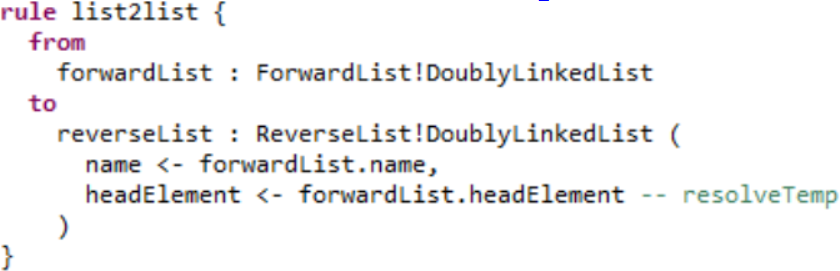
\includegraphics[width=0.75\textwidth]{atl.png}
	\caption{Example using ATL.}
	\label{fig:atl}
\end{figure}

 Modeling the overlaps is difficult, if not impossible, without introducing new objects to identify each pattern of source and target elements. QVTc (and QVTr) therefore introduce an additional trace model which comprises a trace class for each pattern, with trace properties to identify the role of each source and target class within the pattern. Each trace class instance therefore groups related source and target elements. Simple UML navigations enforce most of the required relationships. Additional OCL constraints enforce more complex relationships. Figure~\ref{fig:qvtc-qvts} shows the UML Instance Diagram variant that the Eclipse QVTd implementation uses for the example. 

\begin{figure}[h]
	\centering
	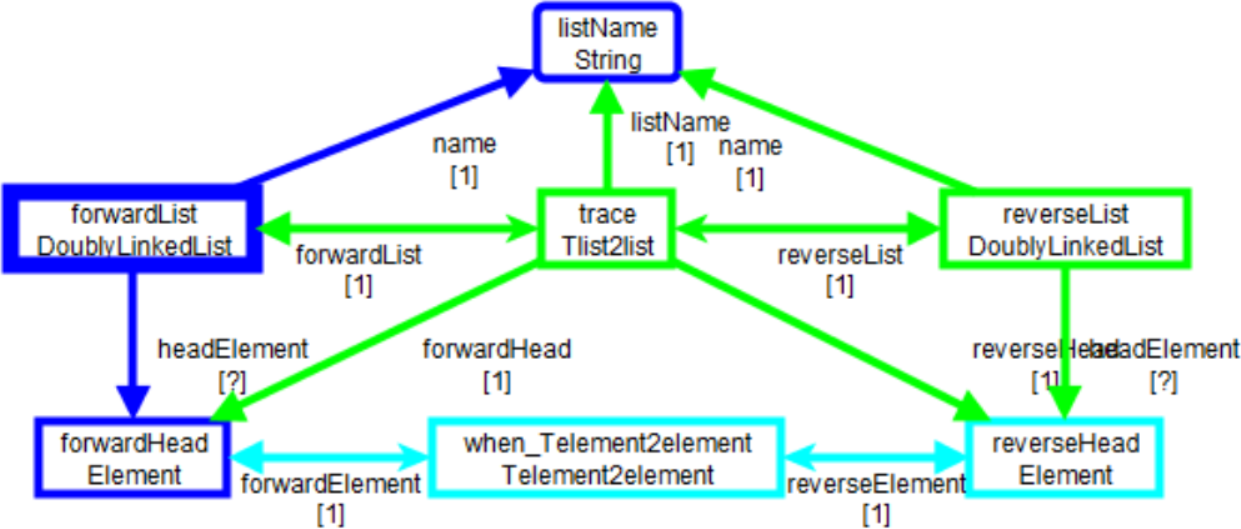
\includegraphics[width=0.9\textwidth]{qvtc-qvts.png}
	\caption{QVTs-like exposition of QVTc mapping.}
	\label{fig:qvtc-qvts}
\end{figure}

The left hand column shows the blue source pattern. The right hand column shows the target pattern. The `copied' value is shared at the top of the middle column. The additional two trace objects in the middle column identify the green creation of a match of the \texttt{list2list} rule using a \texttt{Tlist2list} instance and a cyan dependency on a \texttt{Telement2element} instance, which is  a match of the \texttt{element2element} rule (not  shown).

The transformation author defines the trace model explicitly in QVTc, or implicitly in QVTr. The trace model relates source and target models that are usually developed independently and so the relationships from trace model to source or target model are necessarily unidirectional. There is  no navigable path from \texttt{forwardList} in the source model to \texttt{trace} in the middle model. This conflicts with the bidirectional navigability shown in Figure~\ref{fig:qvtc-qvts} that is necessary to use OCL navigation effectively to define the transformation.

Fortunately, OCL ignores the accidental navigability that may be a deliberate optimization for code generation or the unavoidable consequence of independent model development. In OCL, all object to object properties are navigable in both directions. Where the UML exposition is unidirectional, OCL automatically synthesizes an opposite using the name of the unnavigable target class allowing the use of \texttt{forwardList.Tlist2list}. If the forward name is ambiguous, the opposite name may be used to disambiguate: \texttt{forwardList.Tlist2list[forwardList]}.

The comprehensive opposite navigation capabilities of OCL therefore provide the foundation for the rigorous modeling of a side effect free QVTc or QVTr declarative transformation.
\end{document}
